\documentclass[a4paper,12pt]{article}

\usepackage[utf8x]{inputenc}
\usepackage[T2A]{fontenc}
\usepackage[english, russian]{babel}

% Опционно, требует  apt-get install scalable-cyrfonts.*
% и удаления одной строчки в cyrtimes.sty
% Сточку не удалять!
% \usepackage{cyrtimes}

% Картнки и tikz
\usepackage{graphicx}
\usepackage{tikz}
\usetikzlibrary{snakes,arrows,shapes}


% Некоторая русификация.
\usepackage{misccorr}
\usepackage{indentfirst}
\renewcommand{\labelitemi}{\normalfont\bfseries{--}}

% Увы, поля придётся уменьшить из-за листингов.
\topmargin -1cm
\oddsidemargin -0.5cm
\evensidemargin -0.5cm
\textwidth 17cm
\textheight 24cm

\sloppy

% Оглавление в PDF
\usepackage[
bookmarks=true,
colorlinks=true, linkcolor=black, anchorcolor=black, citecolor=black, menucolor=black,filecolor=black, urlcolor=black,
unicode=true
]{hyperref}

% Для исходного кода в тексте
\newcommand{\Code}[1]{\texttt{#1}}


\title{Отчёт по лабораторной работе \\ <<Динамическая IP-маршрутизация>>}
\author{(Фроловский Алексей Вадимович)}

\begin{document}

\maketitle

\tableofcontents

\section{Настройка сети}

\subsection{Топология сети}

Топология сети и используемые IP-адреса показаны на рисунке~\ref{fig:network}.

\begin{figure}
\centering
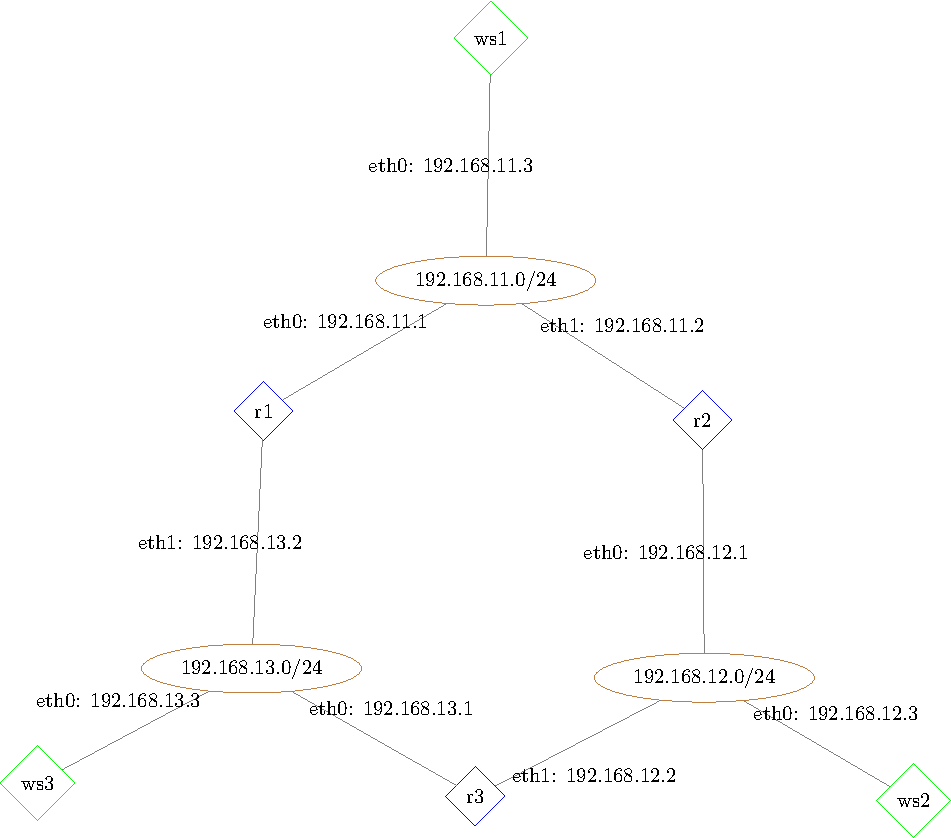
\includegraphics[width=0.8\textwidth]{includes/network_gv.pdf}
\caption{Топология сети}
\label{fig:network}
\end{figure}

На следующих узлах используется динамическая IP-маршрутизация: 
\textbf{r1}, \textbf{r2}, \textbf{r3}, \textbf{r4}, \textbf{r5}, \textbf{wsp1}

\subsection{Назначение IP-адресов}

Ниже приведёны файлы сетевой настройки узлов:
\begin{itemize}

\item маршрутизатор \textbf{r1}
\begin{Verbatim}
auto lo
iface lo inet loopback

auto eth0
iface eth0 inet static
address 10.103.0.1
netmask 255.255.0.0

auto eth1
iface eth1 inet static
address 10.104.0.1
netmask 255.255.0.0
\end{Verbatim}

\item маршрутизатор \textbf{r2}:
\begin{Verbatim}
auto lo
iface lo inet loopback

auto eth0
iface eth0 inet static
address 10.102.0.1
netmask 255.255.0.0

auto eth1
iface eth1 inet static
address 10.103.0.2
netmask 255.255.0.0
\end{Verbatim}

\item маршрутизатор \textbf{r3}:
\begin{Verbatim}
auto lo
iface lo inet loopback

auto eth0
iface eth0 inet static
address 10.101.0.1
netmask 255.255.0.0

auto eth1
iface eth1 inet static
address 10.102.0.2
netmask 255.255.0.0

auto eth2
iface eth2 inet static
address 10.106.0.1
netmask 255.255.0.0
\end{Verbatim}

\item маршрутизатор \textbf{r4}:
\begin{Verbatim}
auto lo
iface lo inet loopback

auto eth0
iface eth0 inet static
address 10.103.0.3
netmask 255.255.0.0

auto eth1
iface eth1 inet static
address 10.105.0.1
netmask 255.255.0.0

auto eth2
iface eth2 inet static
address 10.106.0.2
netmask 255.255.0.0
\end{Verbatim}

\item маршрутизатор \textbf{r5}:
\begin{Verbatim}
auto lo
iface lo inet loopback

auto eth0
iface eth0 inet static
address 10.104.0.2
netmask 255.255.0.0

auto eth1
iface eth1 inet static
address 10.105.0.2
netmask 255.255.0.0
\end{Verbatim}

\item рабочая станция \textbf{ws1}:
\begin{Verbatim}
auto lo
iface lo inet loopback

auto eth0
iface eth0 inet static
address 10.101.0.2
netmask 255.255.0.0
gateway 10.101.0.1
\end{Verbatim}

\item рабочая станция \textbf{wsp1}:
\begin{Verbatim}
auto lo
iface lo inet loopback

auto eth0
iface eth0 inet static
address 10.103.0.4
netmask 255.255.0.0
\end{Verbatim}

\end{itemize}

\subsection{Настройка протокола RIP}

Ниже приведен файл \Code{/etc/quagga/ripd.conf} маршрутизатора \textbf{r1}:

\begin{Verbatim}
router rip

network eth0
network eth1

timers basic 10 60 120

redistribute kernel
redistribute connected

log file /var/log/quagga/ripd.log
\end{Verbatim}

Ниже приведен файл \Code{/etc/quagga/ripd.conf} маршрутизатора \textbf{r2}:

\begin{Verbatim}
router rip

network eth0
network eth1

timers basic 10 60 120

redistribute kernel
redistribute connected

log file /var/log/quagga/ripd.log
\end{Verbatim}

Ниже приведен файл \Code{/etc/quagga/ripd.conf} маршрутизатора \textbf{r3}:

\begin{Verbatim}
router rip

network eth1
network eth2

timers basic 10 60 120

redistribute kernel
redistribute connected

log file /var/log/quagga/ripd.log
\end{Verbatim}

Ниже приведен файл \Code{/etc/quagga/ripd.conf} маршрутизатора \textbf{r4}:

\begin{Verbatim}
router rip

network eth0
network eth1
network eth2

timers basic 10 60 120

redistribute kernel
redistribute connected

log file /var/log/quagga/ripd.log
\end{Verbatim}

Ниже приведен файл \Code{/etc/quagga/ripd.conf} маршрутизатора \textbf{r5}:

\begin{Verbatim}
router rip

network eth0
network eth1

timers basic 10 60 120

redistribute kernel
redistribute connected

log file /var/log/quagga/ripd.log
\end{Verbatim}

Ниже приведен файл \Code{/etc/quagga/ripd.conf} рабочий станции, связанной с несколькими маршрутизаторами \textbf{wsp1}.

\begin{Verbatim}
router rip

network eth0

timers basic 10 60 120

redistribute kernel
redistribute connected

log file /var/log/quagga/ripd.log
\end{Verbatim}


\section{Проверка настройки протокола RIP}

Вывод \textbf{traceroute} от узла \textbf{wsp2} до узла \textbf{ws1} при
нормальной работе сети.

\begin{Verbatim}
traceroute to 10.101.0.2 (10.101.0.2), 64 hops max, 40 byte packets
 1  10.103.0.2  0 ms  0 ms  0 ms
 2  10.102.0.2  0 ms  0 ms  0 ms
 3  10.101.0.2  11 ms  0 ms  0 ms
\end{Verbatim}

Вывод \textbf{traceroute} от \textbf{ws1} такого-то до внешнего IP 195.19.38.2.

\begin{Verbatim}
traceroute to 195.19.38.2 (195.19.38.2), 64 hops max, 40 byte packets
 1  10.101.0.1 (10.101.0.1)  2 ms  1 ms  1 ms
 2  10.102.0.1 (10.102.0.1)  1 ms  1 ms  1 ms
 3  10.103.0.1 (10.103.0.1)  2 ms  2 ms  1 ms
 4  172.16.0.1 (172.16.0.1)  2 ms  1 ms  1 ms
 5  192.168.1.1 (192.168.1.1)  2 ms  4 ms  1 ms
 6  10.176.192.1 (10.176.192.1)  4 ms  3 ms  4 ms
 7  213.85.210.37 (213.85.210.37)  8 ms  3 ms  2 ms
 8  213.85.208.250 (213.85.208.250)  2 ms  6 ms  4 ms
 9  213.85.208.246 (213.85.208.246)  6 ms  15 ms  5 ms
10  193.232.244.44 (193.232.244.44)  5 ms  6 ms  4 ms
11  194.85.40.214 (194.85.40.214)  4 ms  5 ms  7 ms
12  194.190.254.82 (194.190.254.82)  8 ms  60 ms  6 ms
13  195.19.32.146 (195.19.32.146)  19 ms  7 ms  10 ms
14  195.19.38.2 (195.19.38.2)  7 ms  8 ms  11 ms
\end{Verbatim}

Перехваченное сообщение RIP от маршрутизатора \textbf{r4}:

\begin{Verbatim}
Перехваченное сообщение RIP от любого маршрутизатора
IP (tos 0x0, ttl 1, id 0, offset 0, flags [DF], proto UDP (17), length 92) 10.103.0.3.520 > 224.0.0.9.520: 
	RIPv2, Response, length: 64, routes: 3
	  AFI: IPv4:      10.101.0.0/16, tag 0x0000, metric: 2, next-hop: self
	  AFI: IPv4:      10.105.0.0/16, tag 0x0000, metric: 1, next-hop: self[|rip]
\end{Verbatim}

Вывод таблицы RIP.

\begin{Verbatim}
Codes: R - RIP, C - connected, S - Static, O - OSPF, B - BGP
Sub-codes:
      (n) - normal, (s) - static, (d) - default, (r) - redistribute,
      (i) - interface

     Network            Next Hop         Metric From            Tag Time
R(n) 0.0.0.0/0          10.103.0.1            2 10.103.0.1        0 00:54
R(n) 10.101.0.0/16      10.106.0.1            2 10.106.0.1        0 00:57
R(n) 10.102.0.0/16      10.103.0.2            2 10.103.0.2        0 00:54
C(i) 10.103.0.0/16      0.0.0.0               1 self              0
R(n) 10.104.0.0/16      10.103.0.1            2 10.103.0.1        0 00:54
C(i) 10.105.0.0/16      0.0.0.0               1 self              0
C(i) 10.106.0.0/16      0.0.0.0               1 self              0
R(n) 172.16.0.0/16      10.103.0.1            2 10.103.0.1        0 00:54
\end{Verbatim}

Вывод таблицы маршрутизации.

\begin{Verbatim}
10.101.0.0/16 via 10.106.0.1 dev eth2  proto zebra  metric 2 
10.103.0.0/16 dev eth0  proto kernel  scope link  src 10.103.0.3 
10.102.0.0/16 via 10.103.0.2 dev eth0  proto zebra  metric 2 
10.105.0.0/16 dev eth1  proto kernel  scope link  src 10.105.0.1 
10.104.0.0/16 via 10.103.0.1 dev eth0  proto zebra  metric 2 
172.16.0.0/16 via 10.103.0.1 dev eth0  proto zebra  metric 2 
10.106.0.0/16 dev eth2  proto kernel  scope link  src 10.106.0.2 
default via 10.103.0.1 dev eth0  proto zebra  metric 2
\end{Verbatim}

\section{Расщепленный горизонт и испорченные обратные обновления}

Для выполнения данного пункта лабораторной работы будем слушать интерфейс
\textbf{eth0} на маршрутизаторе \textbf{r2}.

С включенным <<расщепленным горизонтом>>:
\begin{Verbatim}
IP (tos 0x0, ttl 1, id 0, offset 0, flags [DF], proto UDP (17), length 132) 10.102.0.1.520 > 224.0.0.9.520: 
	RIPv2, Response, length: 104, routes: 5
	  AFI: IPv4:         0.0.0.0/0 , tag 0x0000, metric: 2, next-hop: self
	  AFI: IPv4:      10.103.0.0/16, tag 0x0000, metric: 1, next-hop: self
	  AFI: IPv4:      10.104.0.0/16, tag 0x0000, metric: 2, next-hop: self
	  AFI: IPv4:      10.105.0.0/16, tag 0x0000, metric: 2, next-hop: self
	  AFI: IPv4:      172.16.0.0/16, tag 0x0000, metric: 2, next-hop: self
IP (tos 0x0, ttl 1, id 0, offset 0, flags [DF], proto UDP (17), length 92) 10.102.0.2.520 > 224.0.0.9.520: 
	RIPv2, Response, length: 64, routes: 3
	  AFI: IPv4:      10.101.0.0/16, tag 0x0000, metric: 1, next-hop: self
	  AFI: IPv4:      10.105.0.0/16, tag 0x0000, metric: 2, next-hop: self
	  AFI: IPv4:      10.106.0.0/16, tag 0x0000, metric: 1, next-hop: self
\end{Verbatim}

С включенными <<испорченными обновлениями>>:
\begin{Verbatim}
IP (tos 0x0, ttl 1, id 0, offset 0, flags [DF], proto UDP (17), length 192) 10.102.0.1.520 > 224.0.0.9.520: 
	RIPv2, Response, length: 164, routes: 8
	  AFI: IPv4:         0.0.0.0/0 , tag 0x0000, metric: 2, next-hop: self
	  AFI: IPv4:      10.101.0.0/16, tag 0x0000, metric: 16, next-hop: 10.102.0.2
	  AFI: IPv4:      10.102.0.0/16, tag 0x0000, metric: 16, next-hop: self
	  AFI: IPv4:      10.103.0.0/16, tag 0x0000, metric: 1, next-hop: self
	  AFI: IPv4:      10.104.0.0/16, tag 0x0000, metric: 2, next-hop: self
	  AFI: IPv4:      10.105.0.0/16, tag 0x0000, metric: 2, next-hop: self
	  AFI: IPv4:      10.106.0.0/16, tag 0x0000, metric: 16, next-hop: 10.102.0.2
	  AFI: IPv4:      172.16.0.0/16, tag 0x0000, metric: 2, next-hop: self
IP (tos 0x0, ttl 1, id 0, offset 0, flags [DF], proto UDP (17), length 92) 10.102.0.2.520 > 224.0.0.9.520: 
	RIPv2, Response, length: 64, routes: 3
	  AFI: IPv4:      10.101.0.0/16, tag 0x0000, metric: 1, next-hop: self
	  AFI: IPv4:      10.105.0.0/16, tag 0x0000, metric: 2, next-hop: self
	  AFI: IPv4:      10.106.0.0/16, tag 0x0000, metric: 1, next-hop: self
\end{Verbatim}

С отключенным <<расщепленным горизонтом>>:
\begin{Verbatim}
IP (tos 0x0, ttl 1, id 0, offset 0, flags [DF], proto UDP (17), length 192) 10.102.0.1.520 > 224.0.0.9.520: 
	RIPv2, Response, length: 164, routes: 8
	  AFI: IPv4:         0.0.0.0/0 , tag 0x0000, metric: 2, next-hop: self
	  AFI: IPv4:      10.101.0.0/16, tag 0x0000, metric: 2, next-hop: 10.102.0.2
	  AFI: IPv4:      10.102.0.0/16, tag 0x0000, metric: 1, next-hop: self
	  AFI: IPv4:      10.103.0.0/16, tag 0x0000, metric: 1, next-hop: self
	  AFI: IPv4:      10.104.0.0/16, tag 0x0000, metric: 2, next-hop: self
	  AFI: IPv4:      10.105.0.0/16, tag 0x0000, metric: 2, next-hop: self
	  AFI: IPv4:      10.106.0.0/16, tag 0x0000, metric: 2, next-hop: 10.102.0.2
	  AFI: IPv4:      172.16.0.0/16, tag 0x0000, metric: 2, next-hop: self
IP (tos 0x0, ttl 1, id 0, offset 0, flags [DF], proto UDP (17), length 92) 10.102.0.2.520 > 224.0.0.9.520: 
	RIPv2, Response, length: 64, routes: 3
	  AFI: IPv4:      10.101.0.0/16, tag 0x0000, metric: 1, next-hop: self
	  AFI: IPv4:      10.105.0.0/16, tag 0x0000, metric: 2, next-hop: self
	  AFI: IPv4:      10.106.0.0/16, tag 0x0000, metric: 1, next-hop: self
\end{Verbatim}

Как видно при использовании <<расщепленного горизонта>> в сообщение не
включаются те маршруты, которые были получены от других маршрутизаторов
с метрикой 1 (т.е. они находятся сами в этих сетях и, соответственно, знают об этом).
При включеном <<испорченном обратном обновлении>> маршрут такие маршруты
включаются в сообщение, но с метрикой 16. А при отключенном <<расщепленном
горизонте>> посылаются сообщения с реальными метриками о всех известных
маршрутах.

\section{Имитация устранимой поломки в сети}

Для того, чтобы выполнить данный пункт лабораторной работы выключим
маршрутизатор \textbf{r4}

Вывод таблицы RIP непосредственно перед истечением таймера устаревания на маршрутизаторе \textbf{r2}:
\begin{Verbatim}
Codes: R - RIP, C - connected, S - Static, O - OSPF, B - BGP
Sub-codes:
      (n) - normal, (s) - static, (d) - default, (r) - redistribute,
      (i) - interface

     Network            Next Hop         Metric From            Tag Time
R(n) 0.0.0.0/0          10.103.0.1            2 10.103.0.1        0 00:56
R(n) 10.101.0.0/16      10.102.0.2            2 10.102.0.2        0 00:48
C(i) 10.102.0.0/16      0.0.0.0               1 self              0
C(i) 10.103.0.0/16      0.0.0.0               1 self              0
R(n) 10.104.0.0/16      10.103.0.1            2 10.103.0.1        0 00:56
R(n) 10.105.0.0/16      10.103.0.3            2 10.103.0.3        0 00:44
R(n) 10.106.0.0/16      10.102.0.2            2 10.102.0.2        0 00:48
R(n) 172.16.0.0/16      10.103.0.1            2 10.103.0.1        0 00:56
\end{Verbatim}

Перестроенная таблица на этом же маршрутизаторе
\begin{Verbatim}
Codes: R - RIP, C - connected, S - Static, O - OSPF, B - BGP
Sub-codes:
      (n) - normal, (s) - static, (d) - default, (r) - redistribute,
      (i) - interface

     Network            Next Hop         Metric From            Tag Time
R(n) 0.0.0.0/0          10.103.0.1            2 10.103.0.1        0 01:00
R(n) 10.101.0.0/16      10.102.0.2            2 10.102.0.2        0 00:55
C(i) 10.102.0.0/16      0.0.0.0               1 self              0
C(i) 10.103.0.0/16      0.0.0.0               1 self              0
R(n) 10.104.0.0/16      10.103.0.1            2 10.103.0.1        0 01:00
R(n) 10.105.0.0/16      10.103.0.1            3 10.103.0.1        0 01:00
R(n) 10.106.0.0/16      10.102.0.2            2 10.102.0.2        0 00:55
R(n) 172.16.0.0/16      10.103.0.1            2 10.103.0.1        0 01:00
\end{Verbatim}

Вывод \textbf{traceroute} от узла r2 такого-то до r5 такого-то после того, как служба RIP перестроила таблицы маршрутизации.
\begin{Verbatim}
traceroute to 10.105.0.2 (10.105.0.2), 64 hops max, 40 byte packets
 1  10.103.0.1 (10.103.0.1)  9 ms  0 ms  0 ms
 2  10.105.0.2 (10.105.0.2)  16 ms  1 ms  1 ms
\end{Verbatim}

\section{Имитация неустранимой поломки в сети}

Для того, чтобы выполнить данный пункт лабораторной работы выключим
маршрутизатор \textbf{r3}.

После чего сеть 10.101.0.0/16 станет недоступной. Рассмотрим таблицы
маршрутизации и некоторые сообщения, из которых видно, что сеть 10.101.0.0/24
помечена метрикой 16, т.к. она является недоступной.

Таблица маршрутизации у маршрутизатора \textbf{r2} примет следующий вид:

\begin{Verbatim}
Codes: R - RIP, C - connected, S - Static, O - OSPF, B - BGP
Sub-codes:
      (n) - normal, (s) - static, (d) - default, (r) - redistribute,
      (i) - interface

     Network            Next Hop         Metric From            Tag Time
R(n) 0.0.0.0/0          10.103.0.1            2 10.103.0.1        0 00:58
R(n) 10.101.0.0/16      10.102.0.2           16 10.102.0.2        0 01:41
C(i) 10.102.0.0/16      0.0.0.0               1 self              0
C(i) 10.103.0.0/16      0.0.0.0               1 self              0
R(n) 10.104.0.0/16      10.103.0.1            2 10.103.0.1        0 00:58
R(n) 10.105.0.0/16      10.103.0.3            2 10.103.0.3        0 00:57
R(n) 10.106.0.0/16      10.103.0.3            2 10.103.0.3        0 00:57
R(n) 172.16.0.0/16      10.103.0.1            2 10.103.0.1        0 00:58
\end{Verbatim}

\begin{Verbatim}
IP (tos 0x0, ttl 1, id 0, offset 0, flags [DF], proto UDP (17), length 112) 10.103.0.1.520 > 224.0.0.9.520: 
	RIPv2, Response, length: 84, routes: 4
	  AFI: IPv4:         0.0.0.0/0 , tag 0x0000, metric: 1, next-hop: self
	  AFI: IPv4:      10.104.0.0/16, tag 0x0000, metric: 1, next-hop: self[|rip]
IP (tos 0x0, ttl 1, id 0, offset 0, flags [DF], proto UDP (17), length 92) 10.103.0.3.520 > 224.0.0.9.520: 
	RIPv2, Response, length: 64, routes: 3
	  AFI: IPv4:      10.101.0.0/16, tag 0x0000, metric: 16, next-hop: self
	  AFI: IPv4:      10.105.0.0/16, tag 0x0000, metric: 1, next-hop: self[|rip]
\end{Verbatim}

Таблица маршрутизации у маршрутизатора \textbf{r4} примет следующий вид:

\begin{Verbatim}
Codes: R - RIP, C - connected, S - Static, O - OSPF, B - BGP
Sub-codes:
      (n) - normal, (s) - static, (d) - default, (r) - redistribute,
      (i) - interface

     Network            Next Hop         Metric From            Tag Time
R(n) 0.0.0.0/0          10.103.0.1            2 10.103.0.1        0 00:55
R(n) 10.101.0.0/16      10.106.0.1           16 10.106.0.1        0 01:19
R(n) 10.102.0.0/16      10.103.0.2            2 10.103.0.2        0 00:52
C(i) 10.103.0.0/16      0.0.0.0               1 self              0
R(n) 10.104.0.0/16      10.103.0.1            2 10.103.0.1        0 00:55
C(i) 10.105.0.0/16      0.0.0.0               1 self              0
C(i) 10.106.0.0/16      0.0.0.0               1 self              0
R(n) 172.16.0.0/16      10.103.0.1            2 10.103.0.1        0 00:55
\end{Verbatim}

\begin{Verbatim}
IP (tos 0x0, ttl 1, id 0, offset 0, flags [DF], proto UDP (17), length 92) 10.103.0.3.520 > 224.0.0.9.520: 
	RIPv2, Response, length: 64, routes: 3
	  AFI: IPv4:      10.101.0.0/16, tag 0x0000, metric: 16, next-hop: self
	  AFI: IPv4:      10.105.0.0/16, tag 0x0000, metric: 1, next-hop: self[|rip]
IP (tos 0x0, ttl 1, id 0, offset 0, flags [DF], proto UDP (17), length 72) 10.103.0.2.520 > 224.0.0.9.520: 
	RIPv2, Response, length: 44, routes: 2
	  AFI: IPv4:      10.101.0.0/16, tag 0x0000, metric: 16, next-hop: self
	  AFI: IPv4:      10.102.0.0/16, tag 0x0000, metric: 1, next-hop: self
IP (tos 0x0, ttl 1, id 0, offset 0, flags [DF], proto UDP (17), length 112) 10.103.0.1.520 > 224.0.0.9.520: 
	RIPv2, Response, length: 84, routes: 4
	  AFI: IPv4:         0.0.0.0/0 , tag 0x0000, metric: 1, next-hop: self
	  AFI: IPv4:      10.104.0.0/16, tag 0x0000, metric: 1, next-hop: self[|rip]
\end{Verbatim}

\end{document}
